\documentclass{beamer}

% packages
\usepackage{graphicx}
  \graphicspath{{figures}}
\usepackage{minted}
\usepackage{amssymb}

% subfig support
\usepackage{caption}
\usepackage{subcaption}

% packages
\usepackage{biblatex}
  \addbibresource{bibliography.bib}
\usepackage[acronym,nomain]{glossaries}
  \setacronymstyle{long-short}
  \newacronym[shortplural={DoFs},longplural={degrees-of-freedom}]
    {dof}{DoF}{degree-of-freedom}
  \newacronym{fem}{FEM}{the finite element method}
  \newacronym{pde}{PDE}{partial differential equation}
  \newacronym[shortplural={FLOPs},longplural={floating-point operations}]
    {flop}{FLOP}{floating-point operation}
  \newacronym{dag}{DAG}{directed acyclic graph}
  \newacronym{dg}{DG}{discontinous Galerkin}
  \newacronym{poset}{poset}{partially-ordered set}
  \newacronym{rcm}{RCM}{reverse Cuthill-McKee}
  \newacronym{dsl}{DSL}{domain-specific language}
  \newacronym{jit}{JIT}{just-in-time}
  \newacronym{ufl}{UFL}{the Unified Form Language}
  \newacronym{tsfc}{TSFC}{the Two-Stage Form Compiler}
\usepackage{graphicx}
  \graphicspath{{figures}}
\usepackage{minted}
\usepackage{todonotes}
\usepackage{hyperref}
\usepackage{subcaption}
\usepackage{amsmath}
% source: https://tex.stackexchange.com/questions/650034/mathbb-font-for-lowercase-letters
\usepackage[bb=libus]{mathalpha}
\usepackage{pgf}
\usepackage{pgfplots}
\usepackage{tikz}
\usepackage{tkz-euclide}
  \usetikzlibrary{arrows,calc,graphs,graphdrawing,positioning,tikzmark,shapes.geometric,patterns.meta,decorations.pathreplacing}
  \usegdlibrary{trees}
  \pgfdeclarelayer{background}
  \pgfsetlayers{background,main}
  \tikzstyle{ptlabel} = [anchor=center, color=black, opacity=1]
  \tikzset{font={\small}}
  \tikzset{label style/.append style={font=\small}}
  % source: https://tex.stackexchange.com/questions/356564/macro-for-rounded-polygon-around-some-nodes
  \def\drawpolygon#1,#2;{
    \begin{pgfonlayer}{background}
        \filldraw[line width=28,join=round](#1.center)foreach\A in{#2}{--(\A.center)}--cycle;
        \filldraw[line width=27,join=round,blue!10](#1.center)foreach\A in{#2}{--(\A.center)}--cycle;
    \end{pgfonlayer}
  }

% theme info
\usetheme{firedrake}

% title info
\title{\texttt{pyop3}: A new domain-specific language for automating high-performance mesh-based simulation codes}
\author{Connor Ward}
\date{January 2023}

% macros

% checkbox
% source https://tex.stackexchange.com/questions/16000/creating-boxed-check-mark
\newcommand{\unchecked}{\makebox[0pt][l]{$\square$}\raisebox{.15ex}{\hspace{0.1em}$\quad$}}
\newcommand{\maybe}{\makebox[0pt][l]{$\square$}\raisebox{.15ex}{\hspace{0.1em}$\lozenge$}}
\newcommand{\checked}{\makebox[0pt][l]{$\square$}\raisebox{.15ex}{\hspace{0.1em}$\checkmark$}}

% hacky way to get \pyop2 and \pyop3 as valid macros
% source: https://tex.stackexchange.com/questions/13290/how-to-define-macros-with-numbers-in-them
\def\pyop#1{\ifnum#1=2 {PyOP2}\else \ifnum#1=3 {\texttt{pyop3}}\fi \fi}

\newcommand{\basichasse}{%
  \begin{scope}[auto,every node/.style={circle,minimum size=20pt,draw,color=black,fill=white}]
    \begin{scope}[yshift=0cm]
      \node (1) [xshift={1*\textwidth/3}] {1};
      \node (2) [xshift={2*\textwidth/3}] {2};
    \end{scope}

    \begin{scope}[yshift=2cm]
      \node (7) [xshift={1*\textwidth/6}] {7};
      \node (8) [xshift={2*\textwidth/6}] {8};
      \node (9) [xshift={3*\textwidth/6}] {9};
      \node (10) [xshift={4*\textwidth/6}] {10};
      \node (11) [xshift={5*\textwidth/6}] {11};
    \end{scope}

    \begin{scope}[yshift=4cm]
      \node (3) [xshift={1*\textwidth/5}] {3};
      \node (4) [xshift={2*\textwidth/5}] {4};
      \node (5) [xshift={3*\textwidth/5}] {5};
      \node (6) [xshift={4*\textwidth/5}] {6};
    \end{scope}

    \draw [-Stealth] (1) -- (7);
    \draw [-Stealth] (1) -- (8);
    \draw [-Stealth] (1) -- (9);
    \draw [-Stealth] (2) -- (9);
    \draw [-Stealth] (2) -- (10);
    \draw [-Stealth] (2) -- (11);
    \draw [-Stealth] (7) -- (3);
    \draw [-Stealth] (7) -- (5);
    \draw [-Stealth] (8) -- (3);
    \draw [-Stealth] (8) -- (4);
    \draw [-Stealth] (9) -- (4);
    \draw [-Stealth] (9) -- (5);
    \draw [-Stealth] (10) -- (4);
    \draw [-Stealth] (10) -- (6);
    \draw [-Stealth] (11) -- (5);
    \draw [-Stealth] (11) -- (6);
  \end{scope}
}

\newcommand{\py}{\mintinline{python}}
\newcommand{\clang}{\mintinline{c}}
\newcommand{\closure}{\mathbb{cl}}
\newcommand{\support}{\mathbb{supp}}
\newcommand{\plexstar}{\mathbb{st}}
\newcommand{\cone}{\mathbb{cone}}

\newcommand{\hdiv}{$H(\mathrm{div})$ }
\newcommand{\hcurl}{$H(\mathrm{curl})$ }

% drawing triangles
\newcommand{\trianglestyles}{%
  \tikzstyle {cellcolor} = [fill=yellow!80];
  \tikzstyle {edgecolor} = [fill=red!60];
  \tikzstyle {vertcolor} = [fill=blue!30];
  \tikzstyle {segment} = [line width=1.2pt];
  \tikzstyle {dof} = [draw=black,line width=1.2pt];
  \tikzstyle {celldof} = [dof,cellcolor];
  \tikzstyle {edgedof} = [dof,edgecolor];
  \tikzstyle {vertdof} = [dof,vertcolor];
  \tikzstyle {doftext} = [font=\bf];
  \tikzstyle {vdof} = [-stealth,draw=red!60,line width=1.9];
}

\newcommand{\stylesegmentsone}{%
  \tkzSetUpStyle[
    postaction=decorate,
    decoration={
      markings,
      mark=at position .53 with {\arrow[very thick]{##1}},
    }
  ]{myarrow}
}

\newcommand{\stylesegmentstwo}{%
  \tkzSetUpStyle[
    postaction=decorate,
    decoration={
      markings,
      mark=at position .78 with {\arrow[very thick]{##1}},
      mark=at position .28 with {\arrow[very thick]{##1}},
    }
  ]{myarrow}
}

\newcommand{\deftriangle}{%
  \trianglestyles
  \tkzDefPoint(0,0){v0}
  \tkzDefShiftPoint[v0](0:2.5){v1}
  \tkzDefShiftPoint[v0](90:2.5){v2}
}

\newcommand{\defsmalltriangle}{%
  \trianglestyles
  \tkzDefPoint(0,0){v0}
  \tkzDefShiftPoint[v0](0:1.5){v1}
  \tkzDefShiftPoint[v0](90:1.5){v2}
}

\newcommand{\drawtriangle}{%
  \deftriangle
  \tkzDrawSegment[myarrow=stealth,segment](v0,v1)
  \tkzDrawSegment[myarrow=stealth,segment](v1,v2)
  \tkzDrawSegment[myarrow=stealth,segment](v0,v2)
}

\newcommand{\drawsmalltriangle}{%
  \defsmalltriangle
  \tkzDrawSegment[myarrow=stealth,segment](v0,v1)
  \tkzDrawSegment[myarrow=stealth,segment](v1,v2)
  \tkzDrawSegment[myarrow=stealth,segment](v0,v2)
}

\newcommand{\drawflippedtriangle}{%
  \deftriangle
  \tkzDrawSegment[myarrow=stealth,segment](v0,v1)
  \tkzDrawSegment[myarrow=stealth,segment](v2,v1)
  \tkzDrawSegment[myarrow=stealth,segment](v0,v2)
}

\newcommand{\mixedstylesetup}{%
  \tikzstyle{v0} = [fill=blue!50];
  \tikzstyle{v1} = [fill=red!65];
}

\begin{document}

\frame{\titlepage}

% \section{Motivation}

\begin{frame}{\pyop2}
  \begin{itemize}
    \item Used for stencil computations
    \item Handles all the mesh data structures
    \item Firedrake applications include residual assembly and interpolation
  \end{itemize}
\end{frame}

\begin{frame}{\pyop2 data model}
  \begin{itemize}
    \item Vector data is stored by \pyop2 \py{Dats}
    \item These associate a fixed inner shape ($d_m$) with a set of possibly unordered nodes ($i_n$)
    \item \py{Mixed Dats} and \py{Dats} for extruded meshes are also possible
  \end{itemize}

  \centering
  \begin{tikzpicture}[y=-1cm,scale=.75]
    \trianglestyles
    \begin{scope}[yshift=0cm]
      \fill[lightgray] (0,0) rectangle(7,1);
      \filldraw[draw=black,vertcolor] (0.5,0) rectangle ++ (1,1);
      \filldraw[draw=black,vertcolor] (1.5,0) rectangle ++ (1,1);
      \filldraw[draw=black,vertcolor] (2.5,0) rectangle ++ (1,1);
      \filldraw[draw=black,vertcolor] (3.5,0) rectangle ++ (1,1);
      \filldraw[draw=black,vertcolor] (4.5,0) rectangle ++ (1,1);
      \filldraw[draw=black,vertcolor] (5.5,0) rectangle ++ (1,1);
      \node[at={(1,.5)}, ptlabel] {$i_6$};
      \node[at={(2,.5)}, ptlabel] {$i_9$};
      \node[at={(3,.5)}, ptlabel] {$i_0$};
      \node[at={(4,.5)}, ptlabel] {$i_3$};
      \node[at={(5,.5)}, ptlabel] {$i_7$};
      \node[at={(6,.5)}, ptlabel] {$i_4$};
      \draw (0,0) -- (7,0);
      \draw (0,1) -- (7,1);
    \end{scope}

    \begin{scope}[yshift=-2cm]
      \begin{scope}[xshift=2cm]
        \filldraw[draw=black,vertcolor] (0,0) rectangle ++ (1,1);
        \filldraw[draw=black,vertcolor] (1,0) rectangle ++ (1,1);
        \node[at={(0.5,.5)}, ptlabel] {$d_0$};
        \node[at={(1.5,.5)}, ptlabel] {$d_1$};

        \draw (.5,-1) -- (0,0);
        \draw (1.5,-1) -- (2,0);
      \end{scope}
    \end{scope}

  \end{tikzpicture}
\end{frame}

\begin{frame}{Introducing \pyop3}
  \begin{itemize}
    \item Domain-specific language embedded in Python for automating stencil computations
    \item Uses code generation to produce fast code
  \end{itemize}

  % "seems straightforward, why is it so hard? -> data layouts are so diverse!"
\end{frame}

\begin{frame}{Stencil library wishlist}

  \textbf{Features:}

  \unchecked Orientation (e.g. unstructured hexes) \\
  \unchecked p-adaptivity \\
  \unchecked Mixed meshes \\

  \textbf{Performance:}

  \unchecked Mesh partial structure (e.g. extruded)\footnotemark \\
  \unchecked Mesh numbering (e.g. DoFs up extruded columns)\footnotemark[\value{footnote}] \\

  \footnotetext{Achievable in \pyop2 but very complicated and hard to extend}
\end{frame}

\begin{frame}
  Claim: \pyop3's new data layout abstraction enables all of these. 
\end{frame}

\begin{frame}[fragile]{Starting simple: P1}
  \begin{columns}
    \begin{column}{.5\textwidth}
      \centering

      \begin{tikzpicture}
        \stylesegmentsone
        \drawtriangle
        \filldraw [vertdof] (v0) node [doftext] {0} circle [radius=7pt];
        \filldraw [vertdof] (v1) node [doftext] {1} circle [radius=7pt];
        \filldraw [vertdof] (v2) node [doftext] {2} circle [radius=7pt];

        \tkzDefBarycentricPoint(v1=1,v2=1) \tkzGetPoint{to}
        \tkzDefShiftPoint[to](.2,.2){to1}

        % \begin{scope}[overlay]
        %   \tkzDefShiftPoint[v0](1.2,-.8){label0}
        %   \node [font=\scriptsize,at={(label0)}] {Reference element};
        %   \draw [-{stealth},draw=red] (label0) -- (v0);
        % \end{scope}

        \begin{scope}[overlay,xshift=4cm,yshift=1cm]
          \drawsmalltriangle
          \filldraw [vertdof] (v0) node [doftext] {$v_3$} circle [radius=7pt];
          \filldraw [vertdof] (v1) node [doftext] {$v_5$} circle [radius=7pt];
          \filldraw [vertdof] (v2) node [doftext] {$v_6$} circle [radius=7pt];

          \tkzDefBarycentricPoint(v0=1,v2=1) \tkzGetPoint{from}
          \tkzDefShiftPoint[from](-.3,0){from1}

          \draw [-{stealth},densely dashed] (from1) to [bend right=35] (to1);
        \end{scope}

      \end{tikzpicture}

      \vspace{4em}

      \begin{tikzpicture}[y=-1cm,scale=.75]
        \trianglestyles
        \begin{scope}[yshift=0cm]
          \fill[lightgray] (0,0) rectangle(7,1);
          \filldraw[draw=black,vertcolor] (0.5,0) rectangle ++ (1,1);
          \filldraw[draw=black,vertcolor] (1.5,0) rectangle ++ (1,1);
          \filldraw[draw=black,vertcolor] (2.5,0) rectangle ++ (1,1);
          \filldraw[draw=black,vertcolor] (3.5,0) rectangle ++ (1,1);
          \filldraw[draw=black,vertcolor] (4.5,0) rectangle ++ (1,1);
          \filldraw[draw=black,vertcolor] (5.5,0) rectangle ++ (1,1);
          \node[at={(1,.5)}, ptlabel] {$v_3$};
          \node[at={(2,.5)}, ptlabel] {$v_4$};
          \node[at={(3,.5)}, ptlabel] {$v_5$};
          \node[at={(4,.5)}, ptlabel] {$v_6$};
          \node[at={(5,.5)}, ptlabel] {$v_7$};
          \node[at={(6,.5)}, ptlabel] {$v_8$};
          \draw (0,0) -- (7,0);
          \draw (0,1) -- (7,1);
        \end{scope}
      \end{tikzpicture}
    \end{column}

    \hfill

    \begin{column}{.5\textwidth}
      \vspace{4em}
      \begin{minted}[
        frame=lines,
        framesep=2mm,
        baselinestretch=1.2,
        bgcolor=lightgray, fontsize=\tiny,
        linenos
      ]{python}
root = (
  MultiAxis()
  .add_part(AxisPart(nverts))
)
      \end{minted}
    \end{column}
  \end{columns}
\end{frame}

\begin{frame}[fragile]{Adding shape: vector P1}
  \begin{columns}
    \begin{column}{.5\textwidth}
      \centering

      \begin{tikzpicture}
        \stylesegmentsone
        \drawtriangle

        \filldraw [vertdof] (v0) ++ (.2,0) node [doftext] {1} circle [radius=7pt];
        \filldraw [vertdof] (v0) ++ (-.2,.1) node [doftext] {0} circle [radius=7pt];

        \filldraw [vertdof] (v1) ++ (.2,0) node [doftext] {3} circle [radius=7pt];
        \filldraw [vertdof] (v1) ++ (-.2,.1) node [doftext] {2} circle [radius=7pt];

        \filldraw [vertdof] (v2) ++ (.2,0) node [doftext] {5} circle [radius=7pt];
        \filldraw [vertdof] (v2) ++ (-.2,.1) node [doftext] {4} circle [radius=7pt];
      \end{tikzpicture}

      \vspace{2em}

      \begin{tikzpicture}[y=-1cm,scale=.75]
        \trianglestyles
        \begin{scope}[yshift=0cm]
          \fill[lightgray] (0,0) rectangle(7,1);
          \filldraw[draw=black,vertcolor] (0.5,0) rectangle ++ (1,1);
          \filldraw[draw=black,vertcolor] (1.5,0) rectangle ++ (1,1);
          \filldraw[draw=black,vertcolor] (2.5,0) rectangle ++ (1,1);
          \filldraw[draw=black,vertcolor] (3.5,0) rectangle ++ (1,1);
          \filldraw[draw=black,vertcolor] (4.5,0) rectangle ++ (1,1);
          \filldraw[draw=black,vertcolor] (5.5,0) rectangle ++ (1,1);
          \node[at={(1,.5)}, ptlabel] {$v_3$};
          \node[at={(2,.5)}, ptlabel] {$v_4$};
          \node[at={(3,.5)}, ptlabel] {$v_5$};
          \node[at={(4,.5)}, ptlabel] {$v_6$};
          \node[at={(5,.5)}, ptlabel] {$v_7$};
          \node[at={(6,.5)}, ptlabel] {$v_8$};
          \draw (0,0) -- (7,0);
          \draw (0,1) -- (7,1);
        \end{scope}

        \begin{scope}[yshift=-2cm]
          \begin{scope}[xshift=2cm]
            \filldraw[draw=black,vertcolor] (0,0) rectangle ++ (1,1);
            \filldraw[draw=black,vertcolor] (1,0) rectangle ++ (1,1);
            \node[at={(0.5,.5)}, ptlabel] {$d_0$};
            \node[at={(1.5,.5)}, ptlabel] {$d_1$};

            \draw (.5,-1) -- (0,0);
            \draw (1.5,-1) -- (2,0);
          \end{scope}
        \end{scope}

      \end{tikzpicture}
    \end{column}

    \hfill

    \begin{column}{.5\textwidth}
      \begin{minted}[
        frame=lines,
        framesep=2mm,
        baselinestretch=1.2,
        bgcolor=lightgray, fontsize=\tiny,
        linenos
      ]{python}
root = (
  MultiAxis()
  .add_part(AxisPart(nverts))
  .add_subaxis(AxisPart(2))
)
      \end{minted}
    \end{column}
  \end{columns}
\end{frame}

\begin{frame}[fragile]{Multiple entities: P2}
  \begin{columns}
    \begin{column}{.5\textwidth}
      \centering

      \begin{tikzpicture}
        \stylesegmentsone
        \drawtriangle

        \filldraw [vertdof] (v0) node [doftext] {0} circle [radius=7pt];
        \filldraw [vertdof] (v1) node [doftext] {1} circle [radius=7pt];
        \filldraw [vertdof] (v2) node [doftext] {2} circle [radius=7pt];

        % edge dofs
        \tkzDefBarycentricPoint(v0=1,v1=1) \tkzGetPoint{e0d0}
        \filldraw [edgedof] (e0d0) node [doftext] {5} circle [radius=7pt];

        \tkzDefBarycentricPoint(v1=1,v2=1) \tkzGetPoint{e1d0}
        \filldraw [edgedof] (e1d0) node [doftext] {3} circle [radius=7pt];

        \tkzDefBarycentricPoint(v0=1,v2=1) \tkzGetPoint{e2d0}
        \filldraw [edgedof] (e2d0) node [doftext] {4} circle [radius=7pt];
      \end{tikzpicture}

      \vspace{2em}

      \begin{tikzpicture}[y=-1cm,scale=.75]
        \trianglestyles
        \begin{scope}[yshift=0cm]
          \fill[lightgray] (0,0) rectangle(7,1);
          \filldraw[draw=black,edgecolor] (0,0) rectangle ++ (1,1);
          \filldraw[draw=black,edgecolor] (1,0) rectangle ++ (1.5,1);
          \filldraw[draw=black,edgecolor] (2.5,0) rectangle ++ (1,1);
          \filldraw[draw=black,vertcolor] (3.5,0) rectangle ++ (1,1);
          \filldraw[draw=black,vertcolor] (4.5,0) rectangle ++ (1.5,1);
          \filldraw[draw=black,vertcolor] (6,0) rectangle ++ (1,1);
          \node[at={(.5,.5)}, ptlabel] {$e_0$};
          \node[at={(1.75,.5)}, ptlabel] {\dots};
          \node[at={(3,.5)}, ptlabel] {$e_m$};
          \node[at={(4,.5)}, ptlabel] {$v_0$};
          \node[at={(5.25,.5)}, ptlabel] {\dots};
          \node[at={(6.5,.5)}, ptlabel] {$v_n$};
          \draw (0,0) -- (7,0);
          \draw (0,1) -- (7,1);
        \end{scope}
      \end{tikzpicture}
    \end{column}

    \hfill

    \begin{column}{.5\textwidth}
      \checked p-adaptivity \\
      \checked Mixed meshes

      \vspace{2em}

      \begin{minted}[
        frame=lines,
        framesep=2mm,
        baselinestretch=1.2,
        bgcolor=lightgray, fontsize=\tiny,
        linenos
      ]{python}
root = (
  MultiAxis()
  .add_part(AxisPart(nedges))
  .add_part(AxisPart(nverts))
)
      \end{minted}
    \end{column}
  \end{columns}
\end{frame}

\begin{frame}[fragile]{Now with renumbering}
  \begin{columns}
    \begin{column}{.5\textwidth}
      \centering

      \begin{tikzpicture}
        \stylesegmentsone
        \drawtriangle

        \filldraw [vertdof] (v0) node [doftext] {0} circle [radius=7pt];
        \filldraw [vertdof] (v1) node [doftext] {1} circle [radius=7pt];
        \filldraw [vertdof] (v2) node [doftext] {2} circle [radius=7pt];

        % edge dofs
        \tkzDefBarycentricPoint(v0=1,v1=1) \tkzGetPoint{e0d0}
        \filldraw [edgedof] (e0d0) node [doftext] {5} circle [radius=7pt];

        \tkzDefBarycentricPoint(v1=1,v2=1) \tkzGetPoint{e1d0}
        \filldraw [edgedof] (e1d0) node [doftext] {3} circle [radius=7pt];

        \tkzDefBarycentricPoint(v0=1,v2=1) \tkzGetPoint{e2d0}
        \filldraw [edgedof] (e2d0) node [doftext] {4} circle [radius=7pt];
      \end{tikzpicture}

      \vspace{2em}

      \begin{tikzpicture}[y=-1cm,scale=.75]
        \trianglestyles
        \begin{scope}[yshift=0cm]
          \fill[lightgray] (0,0) rectangle(7,1);
          \filldraw[draw=black,edgecolor] (0.5,0) rectangle ++ (1,1);
          \filldraw[draw=black,vertcolor] (1.5,0) rectangle ++ (1,1);
          \filldraw[draw=black,edgecolor] (2.5,0) rectangle ++ (1,1);
          \filldraw[draw=black,edgecolor] (3.5,0) rectangle ++ (1,1);
          \filldraw[draw=black,vertcolor] (4.5,0) rectangle ++ (1,1);
          \filldraw[draw=black,vertcolor] (5.5,0) rectangle ++ (1,1);
          \node[at={(1,.5)}, ptlabel] {$e_2$};
          \node[at={(2,.5)}, ptlabel] {$v_7$};
          \node[at={(3,.5)}, ptlabel] {$e_1$};
          \node[at={(4,.5)}, ptlabel] {$e_0$};
          \node[at={(5,.5)}, ptlabel] {$v_4$};
          \node[at={(6,.5)}, ptlabel] {$v_2$};
          \draw (0,0) -- (7,0);
          \draw (0,1) -- (7,1);
        \end{scope}
      \end{tikzpicture}
    \end{column}

    \hfill

    \begin{column}{.5\textwidth}
      \checked Mesh numbering

      \vspace{2em}

      \begin{minted}[
        frame=lines,
        framesep=2mm,
        baselinestretch=1.2,
        bgcolor=lightgray, fontsize=\tiny,
        linenos
      ]{python}
root = (
  MultiAxis()
  .add_part(AxisPart(
    nedges,
    numbering=[4,2,5,...],
  ))
  .add_part(AxisPart(
    nverts,
    numbering=[3,0,1,...],
  ))
)
      \end{minted}
    \end{column}
  \end{columns}
\end{frame}

\begin{frame}[fragile]{More complicated inner shape: P3}
  \begin{columns}
    \begin{column}{.5\textwidth}
      \centering

      \begin{tikzpicture}
        \stylesegmentsone
        \drawtriangle

        \filldraw [vertdof] (v0) node [doftext] {0} circle [radius=7pt];
        \filldraw [vertdof] (v1) node [doftext] {1} circle [radius=7pt];
        \filldraw [vertdof] (v2) node [doftext] {2} circle [radius=7pt];

        % edge dofs
        \tkzDefBarycentricPoint(v0=2.3,v1=1) \tkzGetPoint{e0d0}
        \filldraw [edgedof] (e0d0) node [doftext] {7} circle [radius=7pt];

        \tkzDefBarycentricPoint(v0=1,v1=2.3) \tkzGetPoint{e0d1}
        \filldraw [edgedof] (e0d1) node [doftext] {8} circle [radius=7pt];

        \tkzDefBarycentricPoint(v1=2.3,v2=1) \tkzGetPoint{e1d0}
        \filldraw [edgedof] (e1d0) node [doftext] {3} circle [radius=7pt];

        \tkzDefBarycentricPoint(v1=1,v2=2.3) \tkzGetPoint{e1d1}
        \filldraw [edgedof] (e1d1) node [doftext] {4} circle [radius=7pt];

        \tkzDefBarycentricPoint(v0=2.3,v2=1) \tkzGetPoint{e2d0}
        \filldraw [edgedof] (e2d0) node [doftext] {5} circle [radius=7pt];

        \tkzDefBarycentricPoint(v0=1,v2=2.3) \tkzGetPoint{e2d1}
        \filldraw [edgedof] (e2d1) node [doftext] {6} circle [radius=7pt];

        % cell dof
        \tkzDefBarycentricPoint(v0=1,v1=1,v2=1) \tkzGetPoint{c0d0}
        \filldraw [celldof] (c0d0) node [doftext] {9} circle [radius=7pt];
      \end{tikzpicture}

      \vspace{2em}

      \begin{tikzpicture}[y=-1cm,scale=.75]
        \trianglestyles
        \begin{scope}[yshift=0cm]
          \fill[lightgray] (0,0) rectangle(7,1);
          \filldraw[draw=black,vertcolor] (0.5,0) rectangle ++ (1,1);
          \filldraw[draw=black,cellcolor] (1.5,0) rectangle ++ (1,1);
          \filldraw[draw=black,vertcolor] (2.5,0) rectangle ++ (1,1);
          \filldraw[draw=black,edgecolor] (3.5,0) rectangle ++ (1,1);
          \filldraw[draw=black,edgecolor] (4.5,0) rectangle ++ (1,1);
          \filldraw[draw=black,vertcolor] (5.5,0) rectangle ++ (1,1);
          \node[at={(1,.5)}, ptlabel] {$v_5$};
          \node[at={(2,.5)}, ptlabel] {$c_1$};
          \node[at={(3,.5)}, ptlabel] {$v_4$};
          \node[at={(4,.5)}, ptlabel] {$e_4$};
          \node[at={(5,.5)}, ptlabel] {$e_1$};
          \node[at={(6,.5)}, ptlabel] {$v_2$};
          \draw (0,0) -- (7,0);
          \draw (0,1) -- (7,1);
        \end{scope}

        \begin{scope}[yshift=-2cm]
          \begin{scope}[xshift=1.5cm]
            \filldraw[draw=black,cellcolor] (0,0) rectangle ++ (1,1);
            \node[at={(0.5,.5)}, ptlabel] {$d_0$};

            \draw (0,-1) -- (0,0);
            \draw (1,-1) -- (1,0);
          \end{scope}

          \begin{scope}[xshift=3cm]
            \filldraw[draw=black,edgecolor] (0,0) rectangle ++ (1,1);
            \filldraw[draw=black,edgecolor] (1,0) rectangle ++ (1,1);
            \node[at={(0.5,.5)}, ptlabel] {$d_0$};
            \node[at={(1.5,.5)}, ptlabel] {$d_1$};

            \draw (.5,-1) -- (0,0);
            \draw (1.5,-1) -- (2,0);
          \end{scope}
          \begin{scope}[xshift=5.5cm]
            \filldraw[draw=black,vertcolor] (0,0) rectangle ++ (1,1);
            \node[at={(0.5,.5)}, ptlabel] {$d_0$};

            \draw (0,-1) -- (0,0);
            \draw (1,-1) -- (1,0);
          \end{scope}
        \end{scope}

      \end{tikzpicture}
    \end{column}

    \hfill

    \begin{column}{.5\textwidth}
      \begin{minted}[
        frame=lines,
        framesep=2mm,
        baselinestretch=1.2,
        bgcolor=lightgray, fontsize=\tiny,
        linenos
      ]{python}
root = (
  MultiAxis()
  .add_part(AxisPart(ncells, "cells"))
  .add_part(AxisPart(nedges, "edges"))
  .add_part(AxisPart(nverts, "verts"))
  .add_subaxis("edges", AxisPart(2))
)
      \end{minted}
    \end{column}
  \end{columns}
\end{frame}

\begin{frame}[fragile]{Mixed}
      \centering

      \begin{tikzpicture}[y=-1cm,scale=.75]
        \trianglestyles
        \mixedstylesetup
        \begin{scope}[xshift=3.25cm, yshift=0cm]
          \filldraw[fill=white,draw=black] (0,0) rectangle (1,1);
          \filldraw[fill=white,draw=black] (1,0) rectangle (2,1);
          \node[at={(.5,.5)}, ptlabel] {$V_0$};
          \node[at={(1.5,.5)}, ptlabel] {$V_1$};
        \end{scope}

        \begin{scope}[yshift=-2cm]
          \begin{scope}[xshift=0cm]
            \fill[lightgray] (0,0) rectangle (4,1);
            \filldraw[draw=black,cellcolor] (0.5,0) rectangle (1.5,1);
            \filldraw[draw=black,vertcolor] (1.5,0) rectangle (2.5,1);
            \filldraw[draw=black,edgecolor] (2.5,0) rectangle (3.5,1);
            \node[at={(1,.5)},ptlabel] {$c_0$};
            \node[at={(2,.5)},ptlabel] {$v_1$};
            \node[at={(3,.5)},ptlabel] {$e_1$};
            \draw (0,0) -- (4,0);
            \draw (0,1) -- (4,1);
          \end{scope}

          \begin{scope}[xshift=4.5cm]
            \fill[lightgray] (0,0) rectangle (4,1);
            \filldraw[draw=black,cellcolor] (0.5,0) rectangle (1.5,1);
            \filldraw[draw=black,vertcolor] (1.5,0) rectangle (2.5,1);
            \filldraw[draw=black,edgecolor] (2.5,0) rectangle (3.5,1);
            \node[at={(1,.5)},ptlabel] {$c_0$};
            \node[at={(2,.5)},ptlabel] {$v_1$};
            \node[at={(3,.5)},ptlabel] {$e_1$};
            \draw (0,0) -- (4,0);
            \draw (0,1) -- (4,1);
          \end{scope}
        \end{scope}

        \draw [densely dashed] (3.25,1) -- (0,2);
        \draw [densely dashed] (4.25,1) -- (4,2);
        \draw [densely dashed] (4.25,1) -- ({0+4.5},2);
        \draw [densely dashed] (5.25,1) -- ({4+4.5},2);
      \end{tikzpicture}

      \centering
      \begin{minipage}{.6\textwidth}
      \begin{minted}[
        frame=lines,
        framesep=2mm,
        baselinestretch=1.2,
        bgcolor=lightgray, fontsize=\tiny,
        linenos
      ]{python}
root = (
  MultiAxis()
  .add_part(AxisPart(1, "V0"))
  .add_part(AxisPart(1, "V1"))
  .add_subaxis("V0", ...)
  .add_subaxis("V1", ...)
)
      \end{minted}
    \end{minipage}
\end{frame}

\begin{frame}{Ragged}

\end{frame}

\begin{frame}{Stencil library wishlist}

  \textbf{Features:}

  \unchecked Orientation \\
  \checked p-adaptivity \\
  \checked Mixed meshes \\

  \textbf{Performance:}

  \unchecked Mesh partial structure \\
  \checked Mesh numbering
\end{frame}

\begin{frame}{Orientation: P3}
  % show canonical and flipped triangles

\end{frame}

\begin{frame}{Orientation: Raviart-Thomas}
  % show canonical and flipped triangles

\end{frame}

\begin{frame}{Partially-structured meshes: extruded}

\end{frame}

\begin{frame}{Stencil library wishlist}
  \textbf{Features:}

  \checked Orientation \\
  \checked p-adaptivity \\
  \checked Mixed meshes \\

  \textbf{Performance:}

  \checked Mesh partial structure \\
  \checked Mesh numbering
\end{frame}


\section{Final bits}

\begin{frame}{Things I missed}
  % also lets us do map and loop composition (e.g. useful for PCPATCH)

  % matrices
  % works in parallel (MPI)
  % should retain existing work in PyOP2 on GPUs and inter-element vectorisation
  % lets us have structured things
  % lets us do cool data structure things with partially structured meshes (esp. extruded)
  % enables other performance improvements you get by modifying data layout
\end{frame}

\begin{frame}{Summary}

\end{frame}

% appendix

\section{Appendix}

\begin{frame}{Partially-structured meshes: refined}

\end{frame}

\begin{frame}{Axis swapping}

\end{frame}

% \begin{frame}
%   \frametitle{PyOP2}
%
%   \large
%   \textit{PyOP2 is a framework for automating mesh-based computations.}
%   \normalsize
%
%   \begin{itemize}
%     \item
%       \textit{``automating"} means \textit{"using code generation"}
%     \item
%       \textit{``mesh-based computations"} = \textit{Next slide...}
%     \item
%       Integral\footnote{Pun intended.} part of the Firedrake finite element system.
%     \item
%       Support for iteration over extruded meshes (discussed later).
%   \end{itemize}
% \end{frame}
%
% \begin{frame}
%   \frametitle{``Mesh-based computations"}
%
%   \begin{enumerate}
%     \item Loop over a set of mesh entities (e.g. cells).
%     \item Gather (pack) local data\footnote{e.g. ``all DoFs contained within the cell's closure"} from global data structure(s) into temporary array(s).
%     \item Execute a local computation on this packed data.
%     \item Scatter (unpack) the result of the local computation back into some global object.
%   \end{enumerate}
% \end{frame}
%
% \begin{frame}
%   \frametitle{DMPlex}
%
%   \begin{itemize}
%     \item
%       PETSc's unstructured mesh topology abstraction.
%     \item
%       Dimension-independent.
%   \end{itemize}
%
%   \begin{figure}
%     \centering
%     \begin{subfigure}[b]{0.6\textwidth}
%       \centering
%       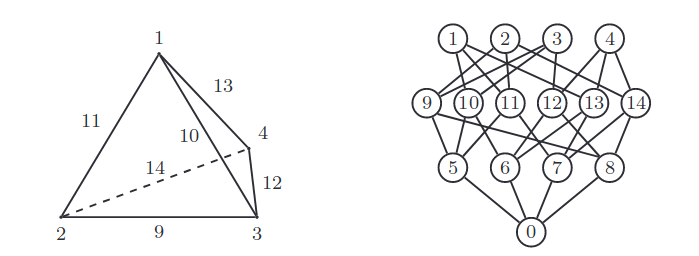
\includegraphics[width=\textwidth]{hasse}
%     \end{subfigure}
%     \\
%     \begin{subfigure}[b]{0.3\textwidth}
%       \centering
%       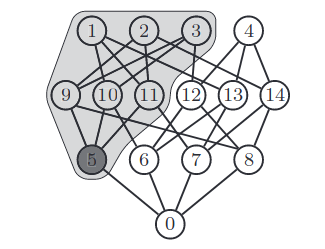
\includegraphics[width=\textwidth]{closure}
%     \end{subfigure}
%     \begin{subfigure}[b]{0.3\textwidth}
%       \centering
%       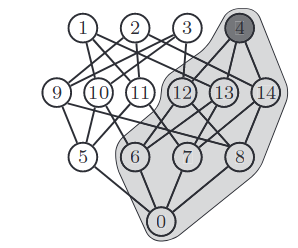
\includegraphics[width=\textwidth]{star}
%     \end{subfigure}
%     \caption{Source: Lange et al. (2016)}
%   \end{figure}
% \end{frame}
%
% \section{What I'm doing}
%
% \begin{frame}
%   \frametitle{\texttt{pyop3}}
%
%   \texttt{pyop3} is a total rewrite of PyOP2 that\dots
%
%   \begin{itemize}
%     \item Has improved composability (e.g. nested loops, map composition, multiple kernels)
%     \item Facilitates some performance optimisations (e.g. loop tiling, loop fusion, data layout transformations)\footnote{Not yet implemented.}
%     \item \textbf{Can generate fast code for a wide variety of composed meshes}
%   \end{itemize}
% \end{frame}
%
% \begin{frame}[containsverbatim]
%   \frametitle{pyop3 interface}
%
%   \tiny
%   \begin{minted}{python}
% # cell assembly
% loop(c := mesh.cells.index, kernel(dat1[closure(c)], dat2[closure(c)]))
%
% # interior facet assembly
% loop(f := mesh.interior_facets.index, [
%   kernel(dat1[closure(support(f))], dat2[closure(support(f))])
% ])
%
% # patches
% loop(v := mesh.verts.index, [
%   loop(p := star(v), kernel(dat1[closure(p)], dat2[closure(p)])),
%   ...
% ])
%   \end{minted}
% \end{frame}
%
% \begin{frame}
%   \frametitle{What does ``fast code" mean?}
%
%   \begin{itemize}
%     \item
%       Accessing data on unstructured meshes is slower than for structured since we need to use indirection maps (i.e. \mintinline{c}{dat[map[i]]} instead of \mintinline{c}{dat[f(i)]}).
%     \item
%     There are circumstances where one can have meshes with structured and unstructured bits (a.k.a. a \textit{composed} mesh).
%     \item
%       We want to be able to generate code that uses direct addressing for the structured parts and indirection maps for the unstructured parts.
%   \end{itemize}
% \end{frame}
%
% \begin{frame}
%   \frametitle{Some example meshes: extruded}
%
%   \begin{itemize}
%     \item
%       Tensor product of an unstructured base mesh with a 1D interval mesh (structured).
%     \item
%       Iteration up columns is fast.
%     \item
%       Hackily supported in PyOP2.
%   \end{itemize}
%
%   \begin{figure}[b]
%     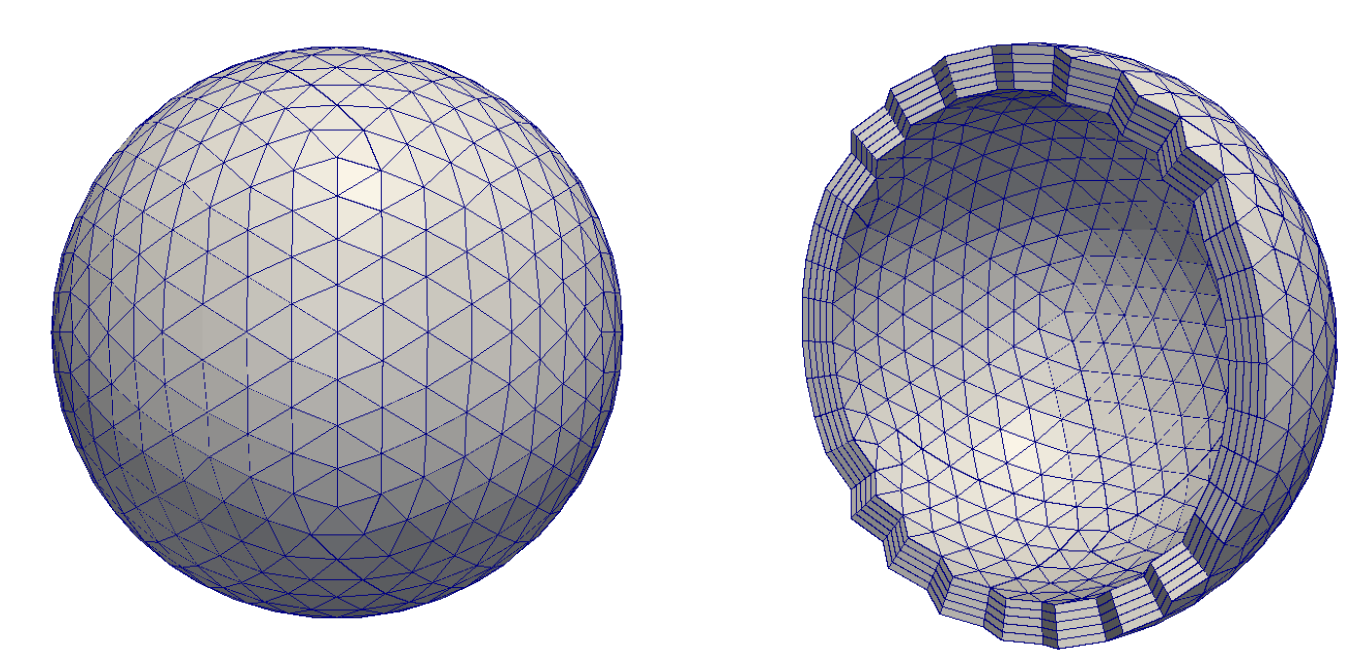
\includegraphics[width=0.7\textwidth]{extruded}
%     \caption{Extruding a sphere (source: firedrakeproject.org).}
%   \end{figure}
% \end{frame}
%
% \begin{frame}
%   \frametitle{Some example meshes: cubed-sphere}
%
%   \begin{itemize}
%     \item
%       Mesh made of 6 structured panels stuck together at the boundaries.
%     \item
%       Looping over the panels is fast.
%   \end{itemize}
%
%   \begin{figure}[b]
%     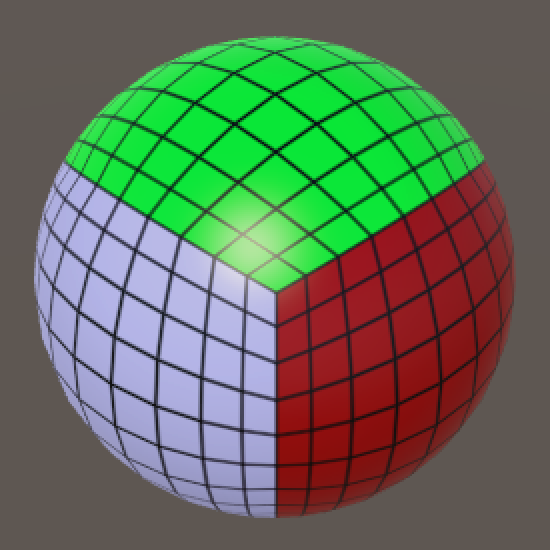
\includegraphics[width=0.45\textwidth]{cubedsphere}
%     \caption{Source: catlikecoding.com}
%   \end{figure}
% \end{frame}
%
% \begin{frame}
%   \frametitle{Some more examples}
%
%   \begin{itemize}
%     \item Block-structured\footnote{I \textit{think} this is the correct term.} (e.g. aerofoils)
%     \item Hybrid
%     \item \textbf{Multigrid?}
%   \end{itemize}
% \end{frame}
%
% \begin{frame}[containsverbatim]
%   \frametitle{Example generated code}
%
%   \tiny
%
%   The pyop3 code:
%
%   \begin{minted}{python}
% loop(
%   c := extruded_mesh.cells.index,
%   [
%     mylocalkernel(dat1[cone(c)], dat2[c])
%   ]
% )
%   \end{minted}
%
%   gets turned into:
%
%   \begin{minted}{c}
% double t0[16];
% double t1[1];
%
% for (int32_t i0 = 0; i0 < ncells; ++i0)  // loop over base cells
%   for (int32_t i1 = 0; i1 < nlayers; ++i1)  // loop up column
%   {
%     for (int32_t i2 = 0; i2 < 3; ++i2)  // loop over cone of base mesh (triangles)
%       for (int32_t i3 = 0; i3 < 2; ++i3)  // loop over cone of interval mesh
%         for (int32_t i4 = 0; i4 < ndofs; ++i4)  // loop over DoFs
%           t0[4 * i2 + 2 * i3 + i4] = dat1[
%             (map0[3 * i0 + i2] * nlayers  // base cone
%             + f(i1, i3)]) * ndofs  // interval cone (no map needed!)
%             + i4  // DoFs
%           ];
%     t1[0] = 0.0;  // initialise output to zero
%     mylocalkernel(&(t0[0]), &(t1[0]));  // local computation
%     dat2[i0 * nlayers + i1] = t1[0];  // write to output
%   \end{minted}
% \end{frame}
%
% \begin{frame}
%   \frametitle{Being rigorous}
%
%   \begin{itemize}
%     \item
%       We want a nice way to describe these sorts of composed meshes such that the code generation can exploit any structure.
%     \item
%       We, possibly erroneously, think that they might form a \textit{ring}.
%       In other words, this would mean that one could \textit{add} and \textit{multiply} meshes with one another.
%     \item
%       For example, an extruded mesh is clearly the product of some base mesh with an interval.
%   \end{itemize}
% \end{frame}
%
% \begin{frame}
%   \frametitle{My questions}
%
%   \begin{itemize}
%     \item
%       Is there a unified way to describe these types of mesh composition?
%     \item
%       How do we propagate structural information such that I can generate code to exploit it?
%     \item
%       Does any of the code I write belong in PETSc instead of pyop3?
%   \end{itemize}
% \end{frame}

\end{document}
